%!TEX root = ../main.tex
%-------------------------------------------------------------------------------
%-------------------------------------------------------------------------------
\begin{frame}\textbf{General setup}\vspace{0.5cm}

\begin{itemize}\setlength\itemsep{1em}
\item joint discussion of research article (45 - 60 minutes)
\item student contributions\medskip
\begin{itemize}\setlength\itemsep{1em}
  \item presentation (20 minutes, up to 10 slides)
  \item lightning talks (5 minutes, no slides)
\end{itemize}
\end{itemize}

\end{frame}
%-------------------------------------------------------------------------------
%-------------------------------------------------------------------------------
\begin{frame}

\begin{itemize}\setlength\itemsep{1em}
  \item Wednesday, noon\medskip
  \begin{itemize}\setlength\itemsep{1em}
    \item deadline for student contributions
    \item announcement of article for joint discussion
    \item selection of student presentation
  \end{itemize}
  \item Monday, lecture\medskip
  \begin{itemize}\setlength\itemsep{1em}
    \item joint discussion
    \item student presentation (peer-grading)
    \item lightning talks
  \end{itemize}
\end{itemize}
\end{frame}
%-------------------------------------------------------------------------------
%-------------------------------------------------------------------------------
\begin{frame}
\textbf{Communication}\\\vspace{0.5cm}
\begin{tabular}{ll}
Slack     & \url{http://bit.ly/human-capital-slack} \\
GitHub    & \url{http://bit.ly/human-capital-github} \\
\end{tabular}
\end{frame}
%-------------------------------------------------------------------------------
%-------------------------------------------------------------------------------
\begin{frame}
\begin{figure}[htp]\centering
\caption{Communications}
\scalebox{0.125}{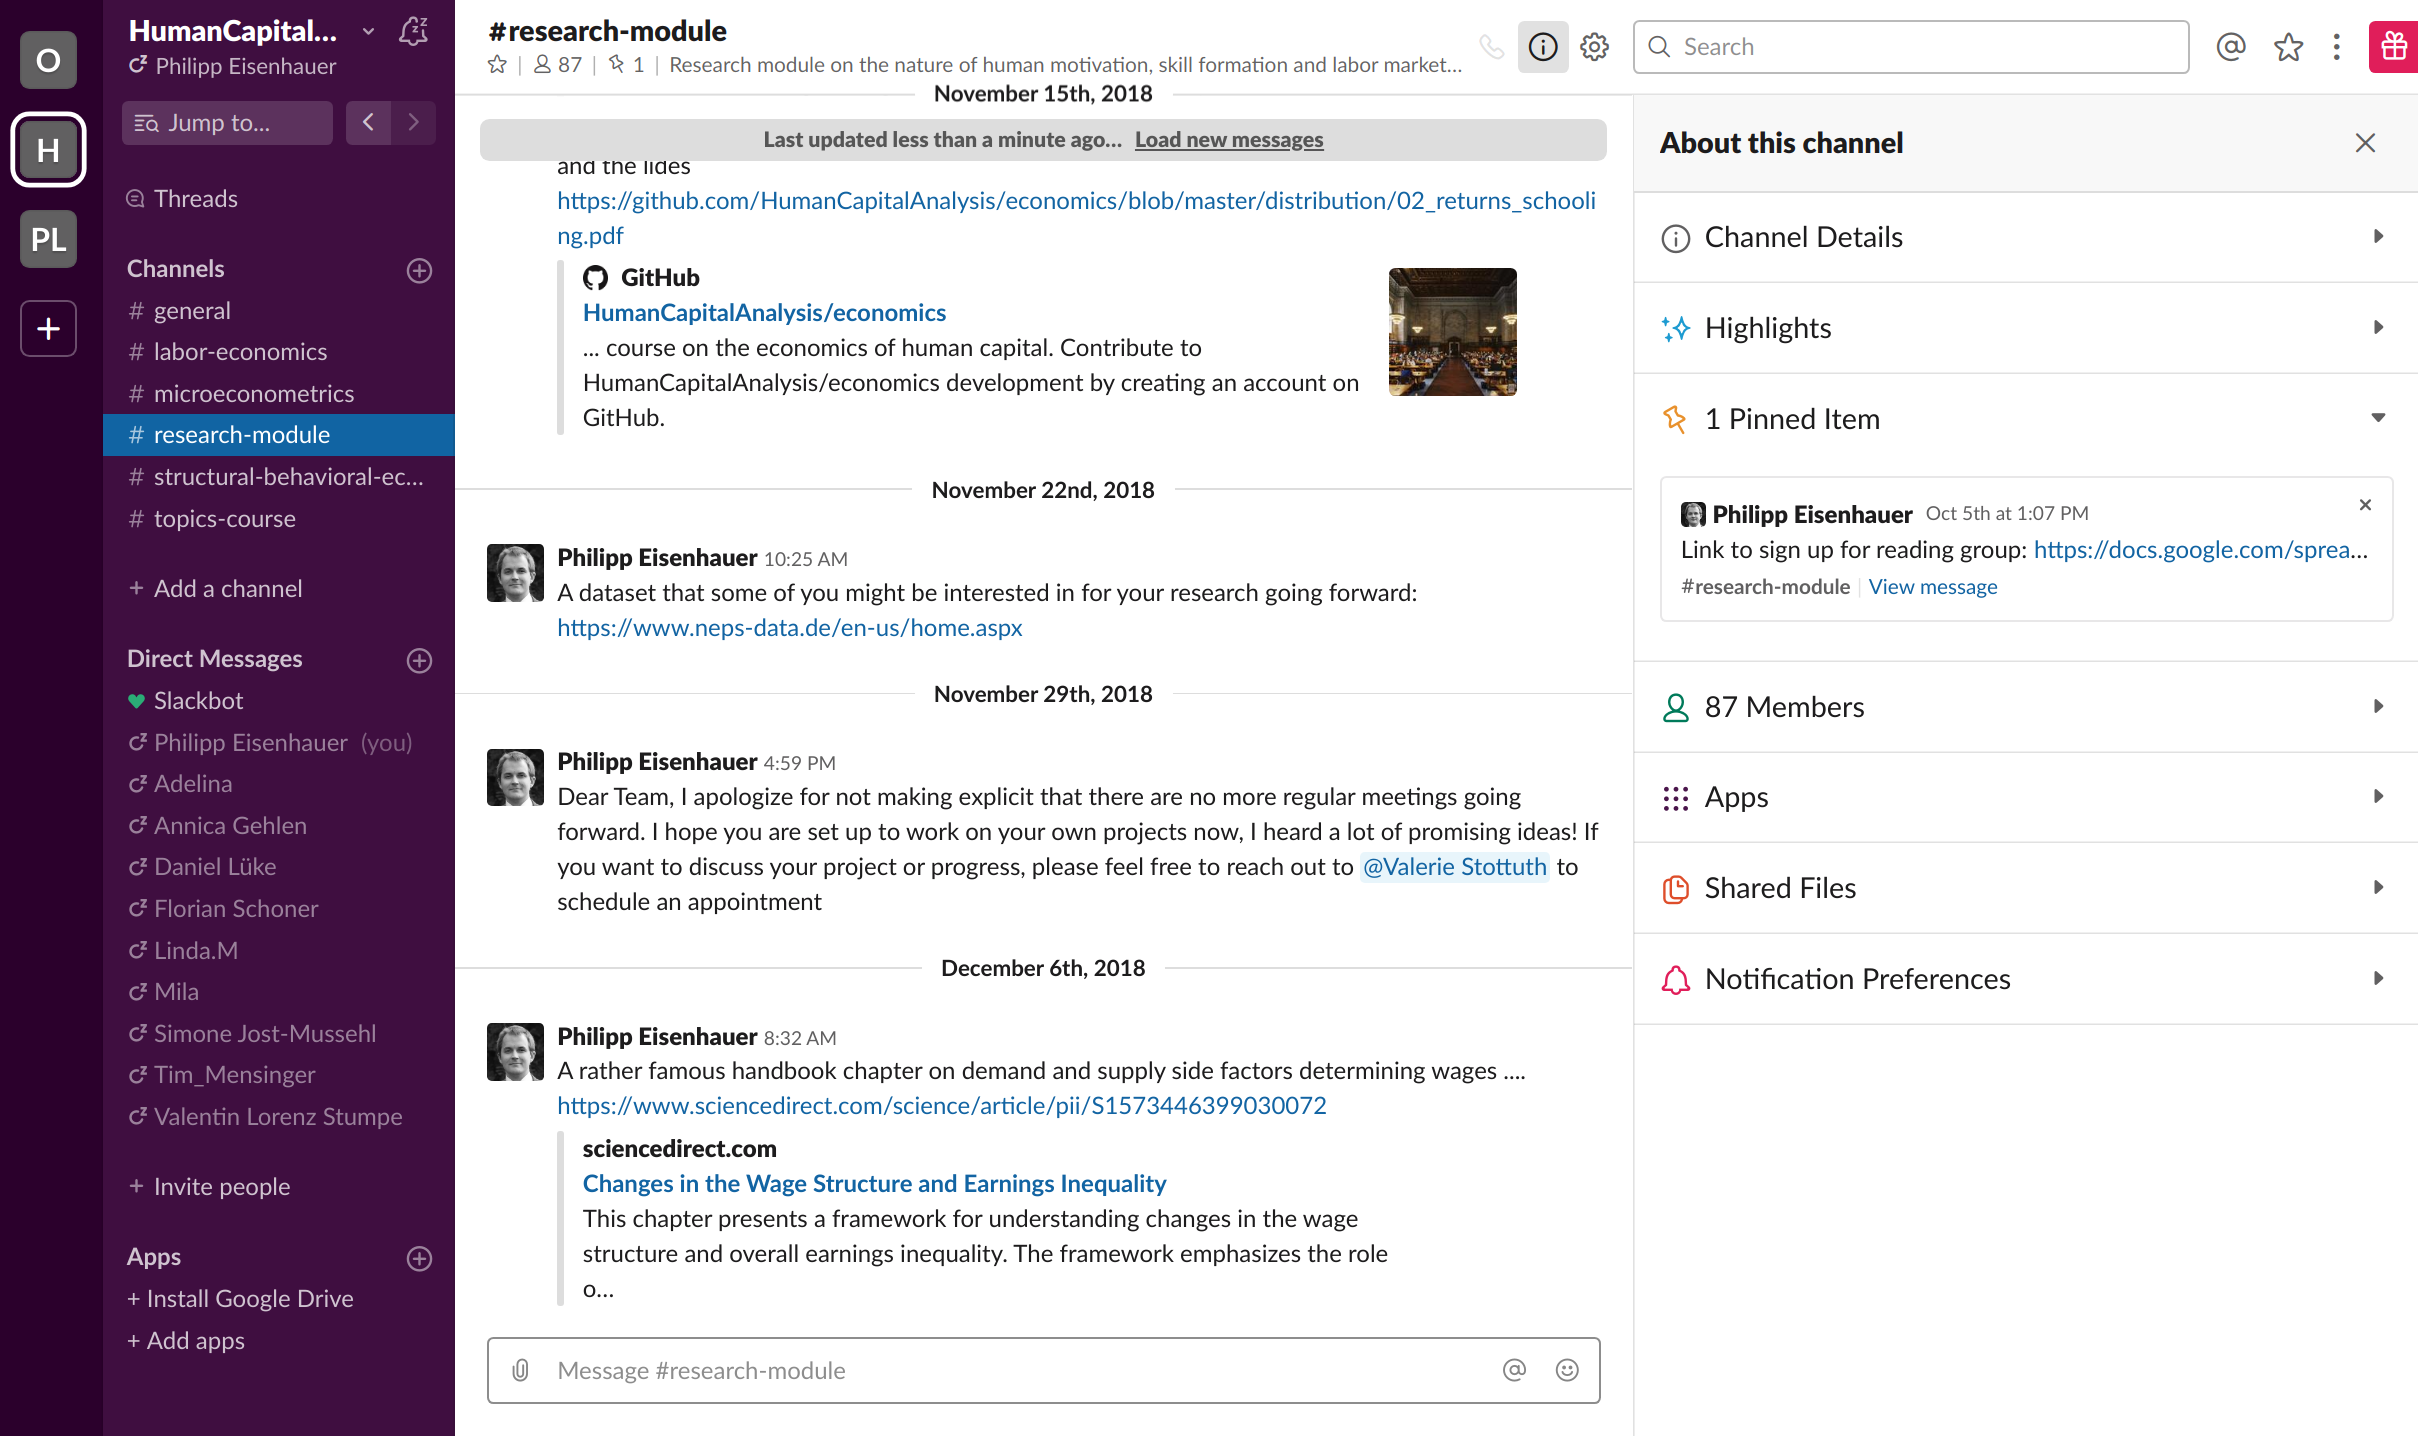
\includegraphics{fig-reading-group-slack}}
\end{figure}
\end{frame}
%-------------------------------------------------------------------------------
%-------------------------------------------------------------------------------
\begin{frame}
\begin{figure}[htp]\centering
\caption{Signup process}
\scalebox{0.20}{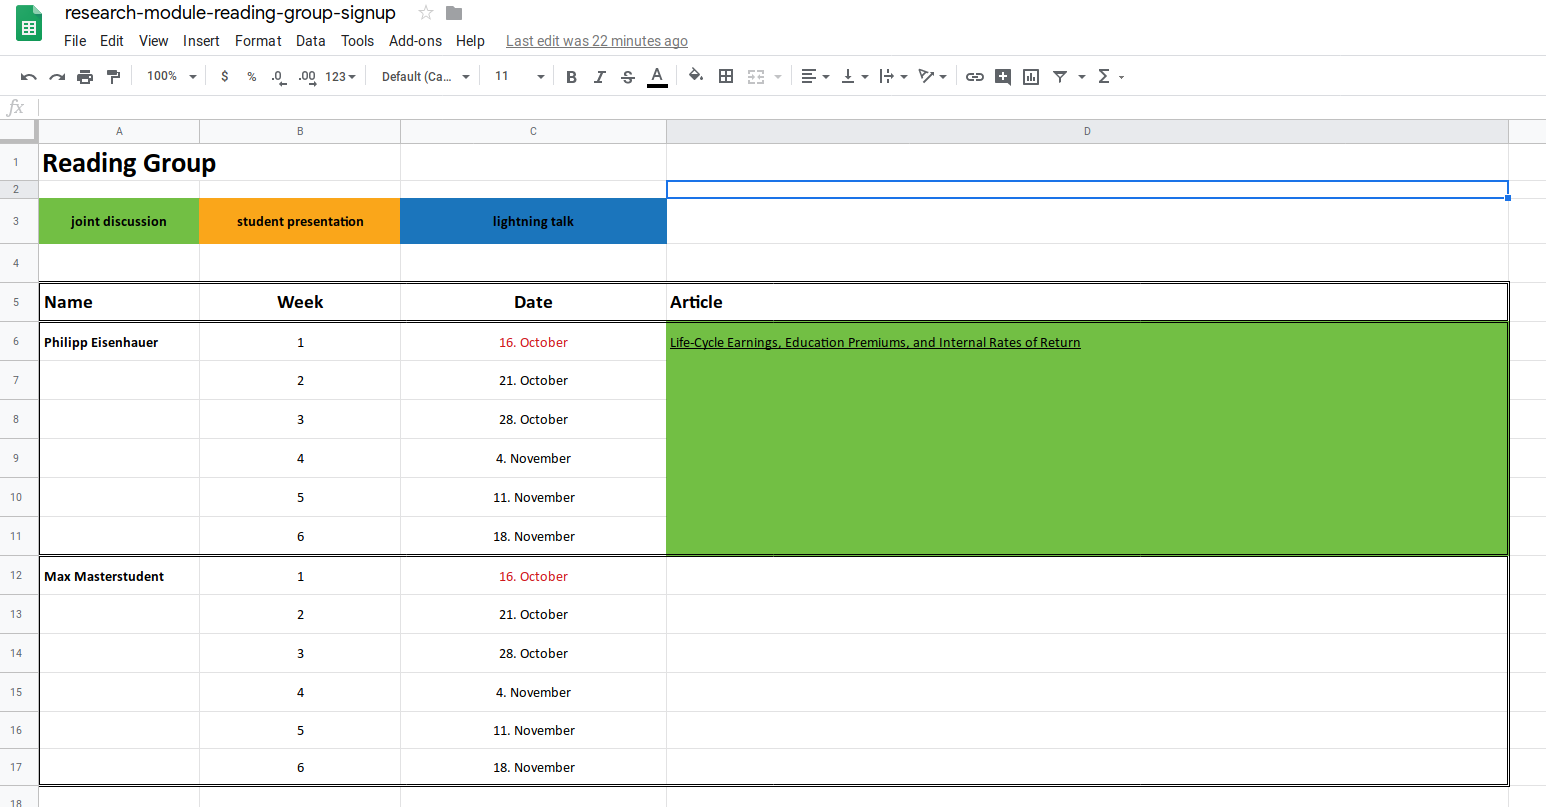
\includegraphics{fig-reading-group-signup}}
\end{figure}
\end{frame}
%-------------------------------------------------------------------------------
%-------------------------------------------------------------------------------
\begin{frame}
\begin{figure}[htp]\centering
\caption{Scientific Reading}
\scalebox{0.35}{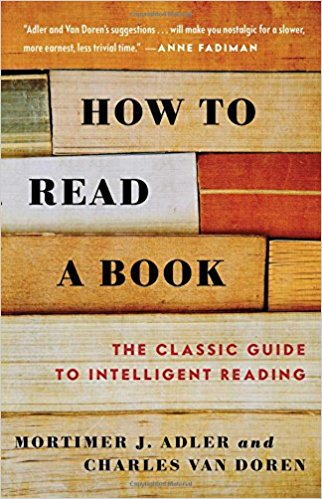
\includegraphics{fig-academic-reading-1}}
\end{figure}
\nocite{Adler.1972}\nocite{Keshav2016}
\end{frame}
%-------------------------------------------------------------------------------
%-------------------------------------------------------------------------------
\begin{frame}

\begin{multicols}{2}
\textbf{Levels of reading}\vspace{0.5cm}
\begin{itemize}\setlength\itemsep{1em}
  \item elementary
  \item inspectional
  \item analytical
  \item syntopical
\end{itemize}

\columnbreak

\textbf{Reading strategies}\vspace{0.5cm}
\begin{itemize}\setlength\itemsep{1em}
\item preview and skim
\item read actively
\item outline and summarize
\item question and wonder
\end{itemize}
\end{multicols}

\end{frame}
%-------------------------------------------------------------------------------
%-------------------------------------------------------------------------------
\begin{frame}\textbf{Start}\vspace{0.5cm}

\begin{itemize}\setlength\itemsep{1em}
\item \bibentry{Mogstad.2017}
\end{itemize}

\end{frame}
%-------------------------------------------------------------------------------
%-------------------------------------------------------------------------------
\begin{frame}\begin{center}
\LARGE\textbf{Conclusion}
\end{center}\end{frame}
